\section{IMPROVEMENTS}
\subsection{Predicted ABM}
\begin{frame}{IMPROVEMENTS}
\framesubtitle{Predicted ABM}
\begin{itemize}
    \item $+$ accuracy $\implies$ $+$ execution time.
    \item ABM converges $\iff$ Predicted ABM converges.
\end{itemize}
    The idea is to calculate different $y _ { h } ^ { \mathrm { p } } \left( t _ { n + 1 } \right)$ until a tolerance is reached, for each instant of time. 
    \begin{center}
    \texttt{y = pabm(f,alpha,y0,T,N,nmax,tol)}
    \end{center}
    For example, using the same Bagley-Torvik equation with larger time step, we have
    \begin{figure}[H]
    \centering
    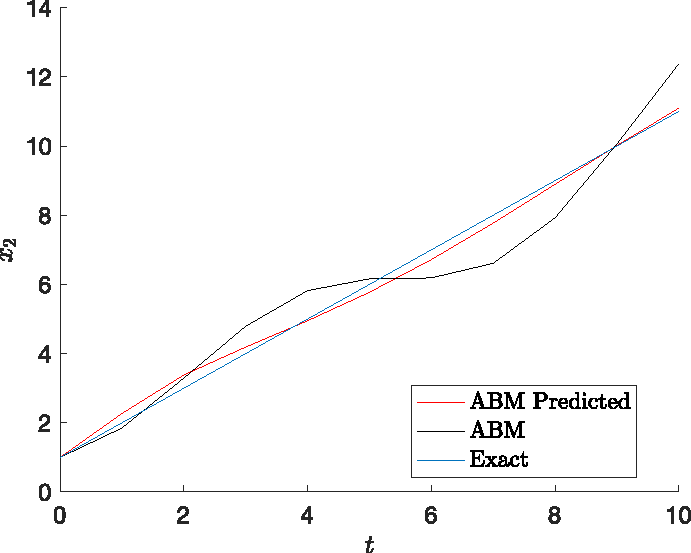
\includegraphics[scale=0.44]{files/mejoras/comparPredictedABM.pdf}
    \caption{Comparison between the original and predicted scheme.}
    \label{fig:comparBagleyTorvik}
\end{figure}
\end{frame}

\subsection{Quadrature Decomposition}
\begin{frame}{IMPROVEMENTS}
\framesubtitle{Quadrature Decomposition}
The idea was to partition the time interval and, on each point, find the polynomial using approximations to the Riemann-Liouville integral.\\[0.4cm]
\begin{center}
    \texttt{y = qDecomposition(f,alpha,y0,N1,N2,T)}
\end{center}
\textbf{Example:}\\[0.4cm]
\begin{multicols}{2}
\begin{equation}
    \begin{cases}
        x'=y&x(0)=1\\
        y'=2x-y&y(0)=-1
    \end{cases}
\end{equation}
\columnbreak
\begin{figure}[H]
    \centering
    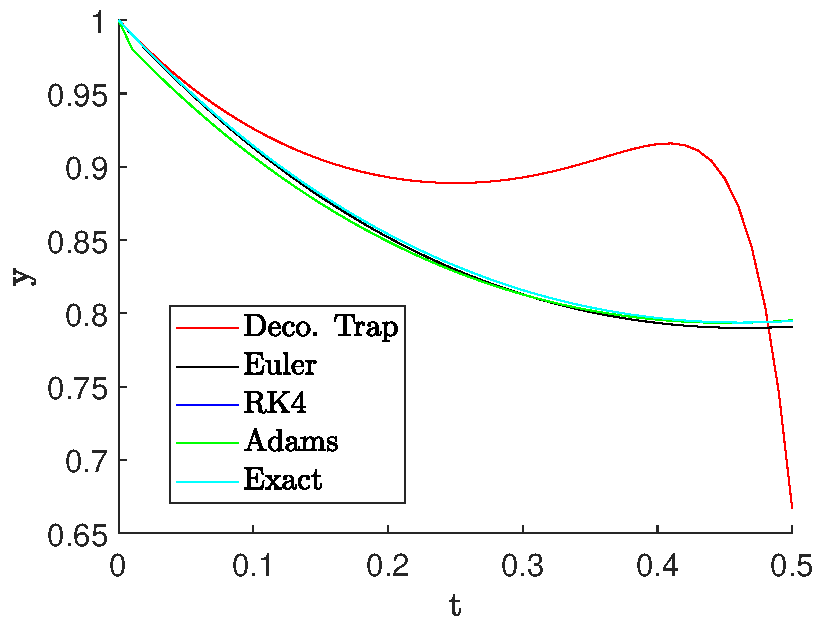
\includegraphics[scale=0.4]{files/mejoras/decom_trap.pdf}
\end{figure}
\end{multicols}
\end{frame}



\subsection{Polynomial Decomposition}
\begin{frame}{IMPROVEMENTS}
\framesubtitle{Polynomial Decomposition}
\begin{itemize}
    \item Analytic solution.
    \item $-$ execution time.
    \item Useful for non-chaotic dynamic systems or chaotic systems for small time frames.
\end{itemize}
The main idea is based on the simple computation of
\begin{equation}
    J^\alpha\left(t^\beta\right)=\dfrac{\Gamma(\beta+1)}{\Gamma(\alpha+\beta+1)}t^{\alpha+\beta}
\end{equation}
which can be extended to non-polynomial expressions using interpolation.

\begin{center}
    \texttt{ySim = pDecomposition(f,alpha,y0,N)}
\end{center}
\end{frame}

\begin{frame}{IMPROVEMENTS}
\framesubtitle{Polynomial Decomposition}
    \textbf{Example:}\\[0.4cm]
    \begin{equation}
        \begin{cases}
        \dfrac{d^3}{dt^3}y(t)+\dfrac{d^{5/2}}{dt^{5/2}}y(t)+y^2(t)=t^4&\\
        y(0)=y'(0)=0,\,y''(0)=2
        \end{cases}
    \end{equation}
    The exact solution is $y(t)=t^2$. Using the procedure for multi-term FDEs, the solution can be approximated as shown in the figure.
    \begin{figure}[H]
        \centering
        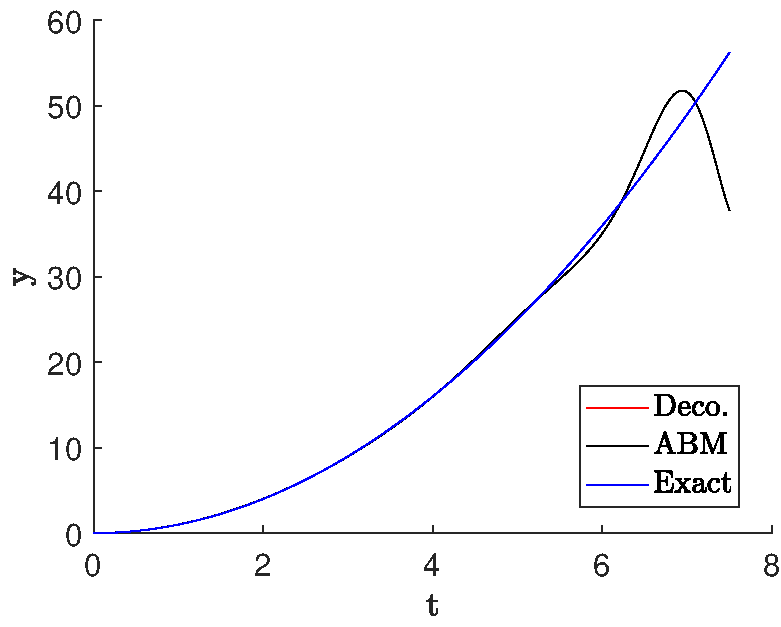
\includegraphics[scale=0.35]{files/mejoras/ABM-vs-Deco-Exact.pdf}
    \end{figure}
\end{frame}

\begin{frame}{IMPROVEMENTS}
\framesubtitle{Polynomial Decomposition}
\textbf{Example: Fractional Lotka-Volterra model}
\begin{equation}
    \begin{cases}{\dfrac{d^{\alpha_1}}{dt^{\alpha_1}}x=\alpha x-\beta x y}& \\[6pt]{\dfrac{d^{\alpha_2}}{dt^{\alpha_2}}y=\delta xy-\gamma y}&\end{cases}
\end{equation}
Using params$=[1,1,1,1]$, c.i$=[1,0.5]$ and $\alpha=[0.5,0.6]$:
\begin{figure}
    \centering
    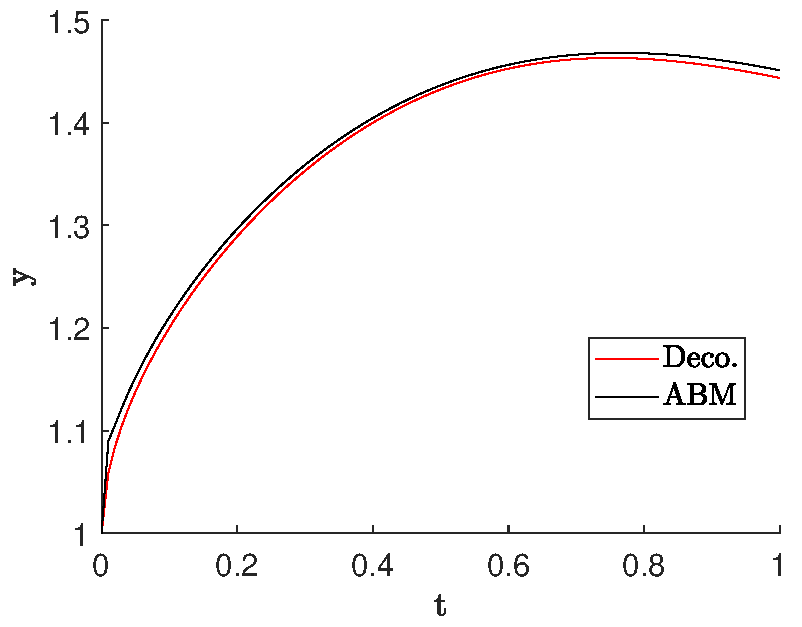
\includegraphics[scale=0.35]{files/mejoras/pred_preey_frac.pdf}
    \end{figure}

\end{frame}

\begin{frame}{IMPROVEMENTS}
\framesubtitle{Polynomial Decomposition}
\textbf{Example: Financial System}
\begin{equation}
    \begin{cases}
    \dfrac{d^{\alpha_1}}{dt^{\alpha_1}} x=z+(y-a)x&\\[6pt]
    \dfrac{d^{\alpha_2}}{dt^{\alpha_2}} y=1-by-x^2&\\[6pt]
    \dfrac{d^{\alpha_3}}{dt^{\alpha_3}} z=-x-cz&
    \end{cases}
\end{equation}
Using params$=[3,0.1,1]$, c.i$=[2,3,2]$ and $\alpha=[1,1,0.8]$, we obtain\begin{multicols}
{2}
\begin{figure}[H]
    \centering
    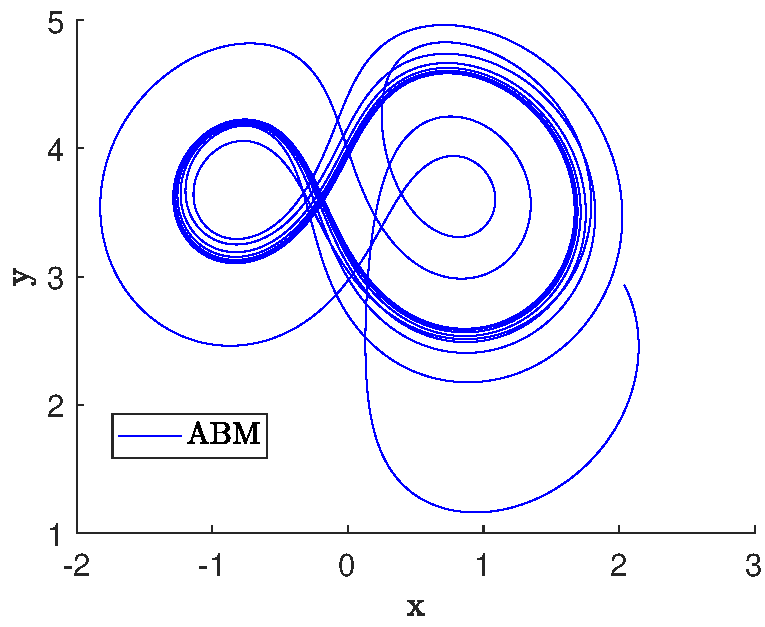
\includegraphics[scale=0.35]{files/comparFrac/finance_chaotic.pdf}
    
\end{figure}
\columnbreak
\begin{figure}[H]
    \centering
    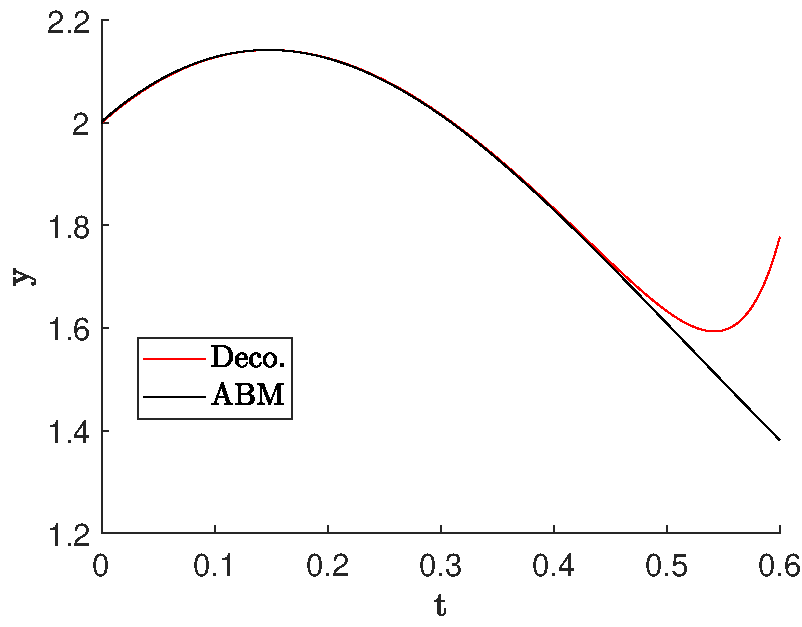
\includegraphics[scale=0.35]{files/mejoras/ABM-vs-Deco-finance.pdf}
\end{figure}
\end{multicols}
\end{frame}

\subsection{Further Work}
\begin{frame}{IMPROVEMENTS}
\framesubtitle{Further Work}
\begin{itemize}
    \item ABM with fixed memory.
    \[\frac { 1 } { \Gamma ( 1 - \alpha ) } \int _ { t - T } ^ { t } \frac { y ^ { \prime } ( s ) } { ( t - s ) ^ { \alpha } } d s\]
    \item ABM with logarithmic memory.
    \[w ^ { p \alpha } \int _ { 0 } ^ { t } \frac { f \left( w ^ { p } x \right) } { ( t - x ) ^ { 1 - \alpha } } d x\]
    \item Richardson extrapolation.
    \[x _ { n } = x \left( t _ { n } \right) + \sum _ { \mu = 1 } ^ { M _ { 1 } } \gamma _ { \mu } n ^ { - \lambda \mu }\]
    \item Decomposition acceleration.
    \[S _ { n } ^ { ( k ) } = \frac { S _ { n } ^ { ( k - 1 ) } S _ { n + 2 } ^ { ( k - 1 ) } - \left( S _ { n + 1 } ^ { ( k - 1 ) } \right) ^ { 2 } } { S _ { n } ^ { ( k - 1 ) } + S _ { n + 2 } ^ { ( k - 1 ) } - 2 S _ { n + 1 } ^ { ( k - 1 ) } } , \quad k \geq 1\]
\end{itemize}
\end{frame}


\section{CONCLUSIONS}
\begin{frame}{CONCLUSIONS}
\begin{multicols}{2}
\begin{itemize}
    \item Fractional calculus $\longrightarrow$ powerful tool to model real and chaotic systems.
    \item Both ABM and decomposition are useful but each with pros and cons.
    \item Both methods can be improved, as shown.
    \item A summary of some essential tools to study fractional systems was successfully constructed.
\end{itemize}
\columnbreak
\begin{figure}[H]
    \centering
    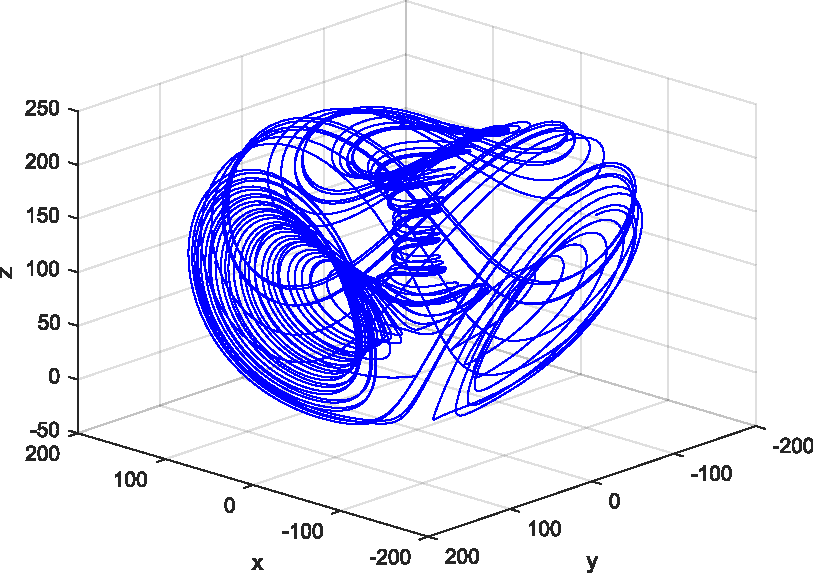
\includegraphics[scale=0.4]{files/3d_chaos.pdf}
\end{figure}
\end{multicols}
\end{frame}